\documentclass[fontset=windows]{article}
\usepackage[margin=1in]{geometry}%设置边距,符合Word设定
\usepackage[UTF8]{ctex}
\usepackage{setspace}
\usepackage{amsmath}
\usepackage{amssymb}
\numberwithin{figure}{section}
\usepackage{array}
\usepackage{lipsum}
\usepackage{float}
\usepackage{graphicx}%插入图片
\usepackage[dvipsnames]{xcolor}
\usepackage{authblk}
\usepackage{listings,matlab-prettifier}
\lstset{
	language=Matlab, % 设置代码语言为Matlab
    basicstyle=\ttfamily, % 设置字体为等宽字体
    numbers=left, % 行号在左边显示
    numberstyle=\tiny, % 设置行号字体大小
    stepnumber=1, % 行号递增步长
    numbersep=5pt, % 行号到代码的距离
    backgroundcolor=\color{gray!10}, % 设置代码的背景颜色
    showspaces=false,
    showstringspaces=false,
    showtabs=false,
    frame=single, % 设置代码框
    rulecolor=\color{black},
    tabsize=2,
    breaklines=true,
    breakatwhitespace=true,
    title=\lstname,
	keywordstyle=\bfseries\color{NavyBlue},
	morekeywords={var,};
	emphstyle=\bfseries\color{Rhodamine}, % 强调词样式设置
    commentstyle=\itshape\color{black!50!white}, % 设置注释样式,斜体,浅灰色
    stringstyle=\bfseries\color{PineGreen!90!black}, % 设置字符串样式
	columns=flexible,}
\graphicspath{{Figures6/}}%文章所用图片在当前目录下的 Figures目录

\usepackage{hyperref} % 对目录生成链接,注:该宏包可能与其他宏包冲突,故放在所有引用的宏包之后
\hypersetup{colorlinks = true,  % 将链接文字带颜色
	linkcolor=black, % 将链接文字黑色
	bookmarksopen = true, % 展开书签
	bookmarksnumbered = true, % 书签带章节编号
	} % 作者
\bibliographystyle{plain}% 参考文献引用格式

\renewcommand{\contentsname}{\centerline{目录}} %经过设置word格式后,将目录标题居中

\title{\heiti\zihao{2} 《统计信号处理》第六教学单元研讨题}
\author{杨 鼎,韦可雷,高司博,高涵博}
\date{}

\begin{document}
\maketitle
\thispagestyle{empty}

%\begin{abstract}
%	\lipsum[2]
%\end{abstract}

%\tableofcontents
%\setcounter{page}{0}
%\newpage

\section{研讨题1}
假设雷达发射信号为线性调频信号\(u(n)=e^{j\pi \mu (nT)^2},|nT_s|\leqslant\frac{T}{2}\),其中\(T\)为脉冲宽度,\(T_s\)为采样间隔,\(\mu=\frac{B}{T}\)为调制斜率,\(B\)为信号带宽。目标距离为\(R\),目标回波幅度为\(A\),雷达接收信号表示为\(z(n)=Au(n-n_0)+w(n),n_0=\frac{2R}{cT_s},w(n)\)服从均值为0,方差为\(\sigma^2\)的高斯白噪声。

1、设\(T=0.1ms,T_s=1.25\times 10^{-7},B=4MHz\)。试设计匹配滤波器,求匹配滤波后目标输出信号表达式,并进行仿真分析。

2、如果存在认为干扰信号,干扰信号形式为\(u_j(n)=A_Je^{}j2\pi f_{JK}\cdot nT_S+j\pi \mu(nT_s)^2,|nT_s|\leqslant\frac{T}{2},f_{JK}=f_{J0}+(k-1)\Delta f_J,\quad k=1,2,3,\cdots,K,f_{J0}=0.5MHz,\Delta f_J=0.4MHz\)。试分析不同\(A_J\)、\(K\)下雷达匹配滤波后的输出信号。

\newpage
\section{研讨题2:雷达信号检测问题。}

对于“\(M/N\)”检测,即\(N\)次独立检测,\(M\)次检测到目标即确定目标存在(虚警类似)。

考虑二元假设
\begin{align*}
    \begin{matrix}
        H_0: & z(k)=n(k)   \\
        H_1: & z(k)=A+n(k)
    \end{matrix}\quad k=0,1,\cdots N-1
\end{align*}
其中噪声\(n(k)\)是服从参量\(\sigma^2\)已知的瑞利分布。

1、对于单个观测数据作为检验统计量,分析检测门限和检测概率;

2、对于N个观测数据进行独立检测,采用“\(1/N\)”检测,分析检测概率及虚警概率。假定单次虚警概率设定为\(0.01,\sigma^2=1,A=1,N=10\),进行仿真分析;

3、若采用“\(2/4\)”检测,要求总体检测概率达到\(0.99\),分析单次检测概率要求,分析虚警概率和单次虚警概率关系。

\subsection*{(1)对于单个观测数据作为检验统计量,分析检测门限和检测概率.}

对于单个观测数据,可以求得NP检验:
\begin{align*}
    L(\mathbf{\mathbf{z}})=\frac{p(\mathbf{x};\mathcal{H}_1)}{p(\mathbf{x};\mathcal{H}_0)}
    =\frac{(z-A)\sigma^{-2}\exp\left[-(z-A)^2\sigma^{-2}\right]}
    {z\sigma^{-2}\exp\left[-z^2\sigma^{-2}\right]}>\gamma
\end{align*}

或者
\begin{align*}
    (1-\frac{A}{z})\exp[\sigma^{-2}(2zA-A^2)]>\gamma
\end{align*}
则判\(\mathcal{H}_1\)。
其中门限\(\gamma\)由
\begin{align*}
    P_{FA}=\int_{\{\mathbf{z}:L(\mathbf{z}>\gamma)\}}p(\mathbf{z};\mathcal{H}_0)d\mathbf{x}
\end{align*}
求出。

将单个观测数据作为检验统计量,即\(T(\mathbf{z})=z\)对于瑞利分布,虚警概率
\begin{align*}
    P_{FA} & =P\{z[0]>\gamma;\mathcal{H}_0\}                                                     \\
           & =\int_{\gamma}^{\infty}p(z[0];\mathcal{H}_0)dz                                      \\
           & =\int_{\gamma}^{\infty}\frac{z}{\sigma^2}\exp \left(-\frac{z^2}{2\sigma^2}\right)dz \\
           & =\exp\left(-\frac{-\gamma^2}{\sigma^2}\right)
\end{align*}

所以检测门限\(\gamma\)为:
\begin{align*}
    \gamma=\sqrt{(-2\sigma^2)\ln P_{FA}}
\end{align*}

检测概率
\begin{align*}
    P_D & =P\{T(\mathbf{z})>\gamma;\mathcal{H}_1\}                                                  \\
        & =\int_{\gamma}^{\infty}p(z;\mathcal{H}_1)dz                                               \\
        & =\int_{\gamma}^{\infty}\frac{(z-A)}{\sigma^2}\exp\left[-\frac{(z-A)^2}{\sigma^2}\right]dz \\
        & =\exp\left(-\frac{(\gamma-A)^2}{2\sigma^2}\right)                                         \\
        & =\exp\left(-\frac{(\sqrt{(-2\sigma^2)\ln P_{FA}}-A)^2}{2\sigma^2}\right)
\end{align*}

随着虚警概率\(P_{FA}\)的增大,检测门限\(\gamma\)逐渐减小。通常虚警概率\(P_{FA}\)很小,\(\sqrt{(-2\sigma^2)\ln P_{FA}}<A\)检测概率\(P_D\)随虚警概率\(P_{FA}\)的增大而增大。

\subsection*{(2)对于N个观测数据进行独立检测,采用“\(1/N\)”检测,分析检测概率及虚警概率。假定单次虚警概率设定为\(0.01,\sigma^2=1,A=1,N=10\),进行仿真分析.}

对于N个观测数据进行独立检测,检测到1次即判\(\mathcal{H}_1\)。

单次观测的虚警概率为\(P(\mathcal{H}_1;\mathcal{H}_0)=P_{FA}\),\(P(\mathcal{H}_0;\mathcal{H}_0)=1-P_{FA}\),对于“\(1/N\)”检测,事件\(\{\mathcal{H}_0;\mathcal{H}_0\}_{1/N}\)需要连续N次单个观测都出现\(\{\mathcal{H}_0;\mathcal{H}_0\}\),即\(P^{1/N}\{\mathcal{H}_0;\mathcal{H}_0\}=[P(\mathcal{H}_0;\mathcal{H}_0)]^N=(1-P_{FA})^N\),所以“\(1/N\)”检测的虚警概率
\begin{align*}
    P^{1/N}_{FA} & =P^{1/N}(\mathcal{H}_1;\mathcal{H}_0)     \\
                 & =1-P^{1/N}\{\mathcal{H}_0;\mathcal{H}_0\} \\
                 & =1-(1-P_{FA})^N
\end{align*}

同理,单次观测的检测概率为\(P(\mathcal{H}_1;\mathcal{H}_1)=P_D\),漏警概率\(P(\mathcal{H}_0;\mathcal{H}_1)=1-P_D\),对于“\(1/N\)”检测,漏警\(\{\mathcal{H}_0;\mathcal{H}_1\}_{1/N}\)需要连续N次单个观测都出现漏警\(\{\mathcal{H}_0;\mathcal{H}_1\}\),即\(P^{1/N}\{\mathcal{H}_0;\mathcal{H}_1\}=[P(\mathcal{H}_0;\mathcal{H}_1)]^N=(1-P_D)^N\),所以“\(1/N\)”检测的检测概率
\begin{align*}
    P^{1/N}_D & =P^{1/N}(\mathcal{H}_1;\mathcal{H}_1)     \\
              & =1-P^{1/N}\{\mathcal{H}_0;\mathcal{H}_1\} \\
              & =1-(1-P_D)^N
\end{align*}

根据第\(\mathbf{(1)}\)问可知
\begin{align*}
    P_D =\exp\left(-\frac{(\sqrt{(-2\sigma^2)\ln P_{FA}}-A)^2}{2\sigma^2}\right)
\end{align*}
所以“\(1/N\)”检测的检测概率为
\begin{align*}
    P^{1/N}_D=1-\left(1-\exp\left(-\frac{(\sqrt{(-2\sigma^2)\ln P_{FA}}-A)^2}{2\sigma^2}\right)\right)^N
\end{align*}

假定单次虚警概率设定为\(0.01,\sigma^2=1,A=1,N=10\),可以计算得到
检测门限为
\begin{align*}
    \gamma & =\sqrt{(-2\sigma^2)\ln P_{FA}} \\
           & =\gamma=\sqrt{-2\ln 0.01}      \\
           & =3.0349
\end{align*}

虚警概率为
\begin{align*}
    P^{1/N}_{FA} & =1-(1-P_{FA})^N  \\
                 & =1-(1-0.01)^{10} \\
                 & =0.0956
\end{align*}

检测概率为
\begin{align*}
    P^{1/N}_D & =1-\left(1-\exp\left(-\frac{(\sqrt{(-2\sigma^2)\ln P_{FA}}-A)^2}{2\sigma^2}\right)\right)^N \\
              & =1-\left(1-\exp\left(-\frac{(\sqrt{(-2)\ln 0.01}-1)^2}{2}\right)\right)^N                   \\
              & =0.7403
\end{align*}

\begin{figure}[H]
    \centering
    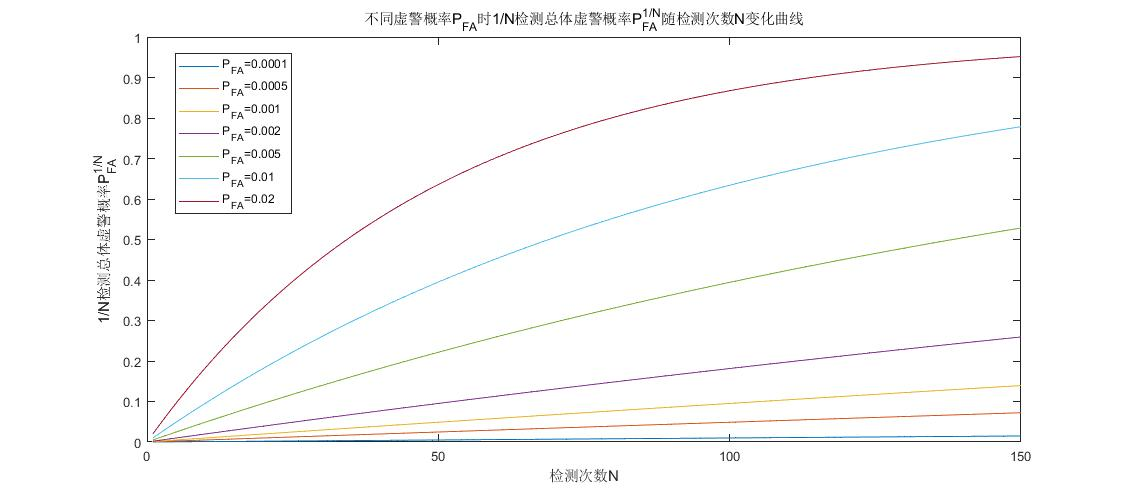
\includegraphics[scale=0.35]{fig2_1.jpg}
    \caption{不同虚警概率\(P_{FA}\)时1/N检测总体虚警概率\(P^{1/N}_{FA}\)随检测次数N变化曲线}
    \label{2.1}
\end{figure}

\begin{figure}[H]
    \centering
    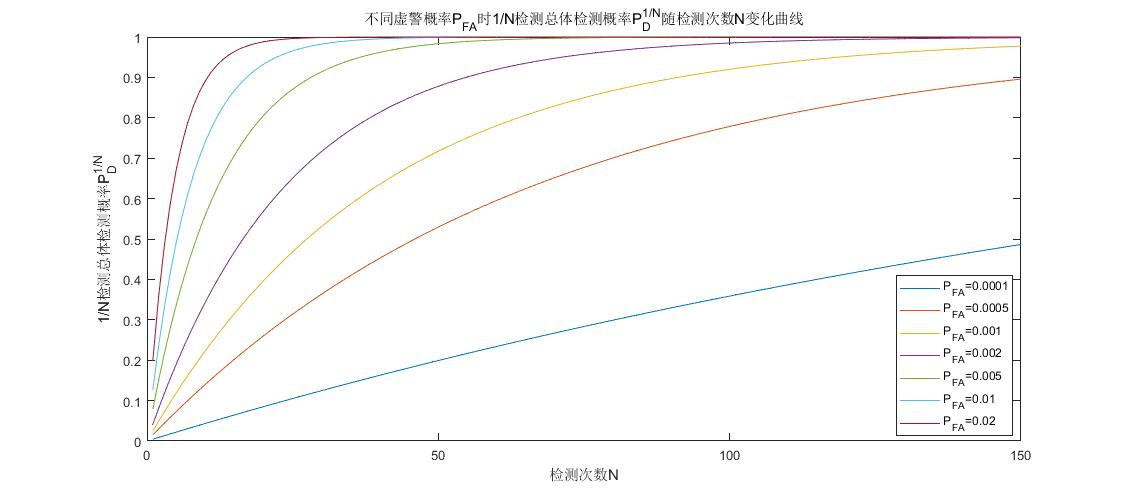
\includegraphics[scale=0.35]{fig2_2.jpg}
    \caption{不同虚警概率\(P_{FA}\)时1/N检测总体检测概率\(P^{1/N}_D\)随检测次数N变化曲线}
    \label{2.2}
\end{figure}

令\(\sigma^2=1,A=1\),当\(P_FA\)等于\(1\times10^{-5},5\times10^{-5},1\times10^{-4},1\times10^{-3},2\times10^{-3},5\times10^{-3},1\times10^{-2},2\times10^{-2}\)时,分别计算总体虚警概率\(P^{1/N}_{FA}\)和总体检测概率\(P^{1/N}_D\)随检测次数N的变化曲线。
得到结果如图\ref*{2.1}和图\ref*{2.2}

对比图\ref*{2.1}和图\ref*{2.2}可以发现,当单次虚警概率\(P_{FA}<0.001\)时,总体虚警概率\(P^{1/N}_{FA}\)随检测次数N增长变化不大,而总体检测概率随检测次数N增长逐渐增加到1。当增加单次虚警概率到\(0.02\)时,虽然总体检测概率在检测次数\(N=20\)时就快速增加到1,但是总体虚警概率\(P^{1/N}_{FA}\)增加也十分快速,\(N=20\)时约为0.34,\(N=100\)时约为0.87,\(N=150\)时约为0.95。所以综合考虑总体虚警概率和总体检测概率,单次虚警概率应当设置为\(P_{FA}=0.001\),检测次数N应当设置在50与100之间,这时总体虚警概率不超过0.1,检测概率在0.7至0.9之间。

\subsection*{(3)若采用“\(2/4\)”检测,要求总体检测概率达到\(0.99\),分析单次检测概率要求,分析虚警概率和单次虚警概率关系}

若采用“\(2/4\)”检测,类似第\(\mathbf{(2)}\)问中分析,检测概率
\begin{align*}
    P^{2/4}_D & =1-(1-P_D)^4-C_4^1P_D(1-P_D)^3 \\
              & =1-(1-P_D)^4-4P_D(1-P_D)^3     \\
              & \geqslant0.99
\end{align*}
解得\(P_D\geqslant 0.8591\),所以单次检测概率的取值范围为\([0.8591,1]\)。

虚警概率\(P^{2/4}_{FA}\)和单次虚警概率\(P_{FA}\)的关系为
\begin{align*}
    P^{2/4}_{FA} & =1-(1-P_{FA})^4-C_4^1P_{FA}(1-P_{FA})^3 \\
                 & =3P_{FA}^4-8P_{FA}^3+6P_{FA}^2
\end{align*}

图\ref*{2.3}画出了虚警概率\(P^{2/4}_{FA}\)随单次虚警概率\(P_{FA}\)变化曲线,并画出了\(6P_{FA}^2\)的变化曲线作为变化趋势的参考。
\begin{figure}[H]
    \centering
    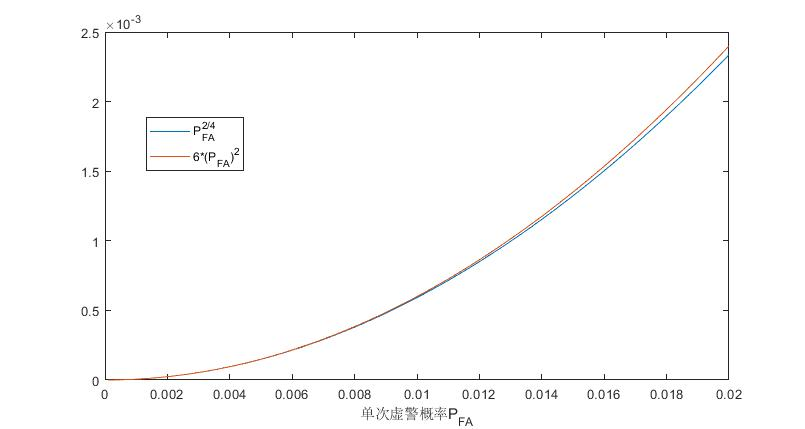
\includegraphics[scale=0.5]{fig2_3.jpg}
    \caption{总体虚警概率\(P^{2/4}_{FA}\)变化趋势比较图}
    \label{2.3}
\end{figure}

\section{研讨题3}

高斯噪声中已知信号的分析与仿真,考虑二元假设
\begin{align*}
    \begin{matrix}
        H_0: & z(k)=n(k)     \\
        H_1: & z(k)=r^k+n(k)
    \end{matrix}\quad k=0,1,\cdots N-1
\end{align*}

1、噪声是服从\(n(k)\sim \mathcal{N}(0,1)\)的WGN,若\(r=0.9,N=20\),虚警概率设定为0.01,分析检测门限及检测概率并仿真;

2、噪声服从\(\mathcal{N}(0,\mathbf{C}),[\mathbf{C}]_{ij}=c[i-j]\),其中\(c[k]=\frac{0.19}{1-0.9^2}0.9^{|k|}\),若\(r=0.9,N=20\),虚警概率设定为\(0.01\),分析检测门限及检测概率并仿真。

\subsection*{(1)噪声是服从\(n(k)\sim \mathcal{N}(0,1)\)的WGN,若\(r=0.9,N=20\),虚警概率设定为0.01,分析检测门限及检测概率并仿真.}

利用NP准则,采用判决式
\begin{align*}
    L(\mathbf{z})=\frac{p(\mathbf{z};\mathcal{H}_0)}{p(\mathbf{z};\mathcal{H}_1)}>\gamma
\end{align*}
则判\(\mathcal{H}_1\)
其中
\begin{align*}
    p(\mathbf{z};\mathcal{H}_0)
     & =\frac{1}{(2\pi\sigma^2)^{N/2}}\exp\left\{-\frac{1}{2\sigma^2}\sum_{k=0}^{N-1}z^2[k]\right\}       \\
    p(\mathbf{z};\mathcal{H}_1)
     & =\frac{1}{(2\pi\sigma^2)^{N/2}}\exp\left\{-\frac{1}{2\sigma^2}\sum_{k=0}^{N-1}(z[k]-r^k)^2\right\} \\
\end{align*}

由此可得
\begin{align*}
    L(\mathbf{z})=\exp\left\{-\frac{1}{2\sigma^2}(-2)\sum_{k=0}^{N-1}r^k(z[k]+\frac{1-r^{2N}}{1-r^2})\right\}>\gamma
\end{align*}
两边取对数
\begin{align*}
    \ln L(\mathbf{z})=\frac{1}{\sigma^2}\sum_{k=0}^{N-1}z[k]r^k-\frac{1}{2\sigma^2}+\frac{1-r^{2N}}{1-r^2}>\ln\gamma
\end{align*}
整理得到
\begin{align*}
    \sum_{k=0}^{N-1}r^kz[k]>\sigma^2 \ln \gamma+\frac{1-r^{2N}}{2(1-r^2)}=\gamma^{\prime}
\end{align*}

令左边为检验统计量\(T(\mathbf{z})\),每种假设下的均值和方差分别为
\begin{align*}
    E[T(\mathbf{z});\mathcal{H}_0]   & =E\left[\sum_{k=0}^{N-1}r^kn(k)\right]=\sum_{k=0}^{N-1}r^kE[n(k)]=0                                \\
    E[T(\mathbf{z};\mathcal{H}_1)]   & =E\left[\sum_{k=0}^{N-1}r^k(r^k+n(k))\right]=\sum_{k=0}^{N-1}r^kE[r^k+n(k)]=\frac{1-r^{2N}}{1-r^2} \\
    Var[T(\mathbf{z});\mathcal{H}_0] & =Var\left(\sum_{k=0}^{N-1}r^kn(k)\right)=\sigma^2\frac{1-r^{2N}}{1-r^2}                            \\
    Var[T(\mathbf{z});\mathcal{H}_0] & =Var\left(\sum_{k=0}^{N-1}r^k(r^k+n(k))\right)=\sigma^2\frac{1-r^{2N}}{1-r^2}
\end{align*}

所以有
\begin{align*}
    T(\mathbf{z})\sim\left\{
    \begin{matrix}
        \mathcal{N}(0,\sigma^2\frac{1-r^{2N}}{1-r^2}),                      & \mathcal{H}_0 \\
        \mathcal{N}(\frac{1-r^{2N}}{1-r^2},\sigma^2\frac{1-r^{2N}}{1-r^2}), & \mathcal{H}_1
    \end{matrix}
    \right.
\end{align*}
可以求得
\begin{align*}
    P_{FA} & =Pr\{T(\mathbf{z})>\gamma^{\prime};\mathcal{H}_0\}=Q\left\{\frac{\gamma^{\prime}\sqrt{1-r^2}}{\sqrt{\sigma^2(1-r^{2N})}}\right\}                                                               \\
    P_D    & =Pr\{T(\mathbf{z})>\gamma^{\prime};\mathcal{H}_1\}=Q\left\{\frac{\gamma^{\prime}\sqrt{1-r^2}}{\sqrt{\sigma^2(1-r^{2N})}}-\frac{\gamma^{\prime}\sqrt{1-r^{2N}}}{\sqrt{\sigma^2(1-r^2)}}\right\}
\end{align*}
由虚警概率可以求得门限
\begin{align*}
    \gamma^{\prime}=\sqrt{\sigma^2\frac{1-r^{2N}}{1-r^2}}Q^{-1}(P_{FA})
\end{align*}
代入\(r=0.9,N=20,P_{FA}=0.01\),可得\(\gamma^{\prime}=5.2973,P_D=0.4804\)。

用MATLAB进行蒙特卡洛仿真,信号长度为20,仿真次数为10000次,仿真得到的阈值和检测概率分布为\(\gamma^{\prime}=5.2974,P_D=0.4831\),与理论值基本一致。

\subsection*{(2)噪声服从\(\mathcal{N}(0,\mathbf{C}),[\mathbf{C}]_{ij}=c[i-j]\),其中\(c[k]=\frac{0.19}{1-0.9^2}0.9^{|k|}\),若\(r=0.9,N=20\),虚警概率设定为\(0.01\),分析检测门限及检测概率并仿真}

噪声协方差矩阵为
\begin{align*}
    \mathbf{C}=
    \begin{bmatrix}
        1         & 0.9       & 0.9^2     & \cdots & 0.9^{N-1} \\
        0.9       & 1         & 0.9       & \cdots & 0.9^{N-2} \\
        0.9^2     & 0.9       & 1         & \cdots & 0.9^{N-3} \\
        \vdots    & \vdots    & \vdots    & \ddots & \vdots    \\
        0.9^{N-1} & 0.9^{N-2} & 0.9^{N-3} & \cdots & 1
    \end{bmatrix}
\end{align*}
利用广义匹配滤波器进行检测,检测器可以表示为:
\begin{align*}
    T(\mathbf{z})=\mathbf{z}^T\mathbf{C}^{-1}\mathbf{s}<\ln \gamma+\frac{1}{2}\mathbf{s}^T\mathbf{C}^{-1}\mathbf{s}=\gamma^{\prime}
\end{align*}
其中\(s(k)=r^k\),检验统计量满足
\begin{align*}
    T(\mathbf{z})\sim\left\{
    \begin{matrix}
        \mathcal{N}(0,\mathbf{s}^T\mathbf{C}^{-1}\mathbf{s}),                                     & \mathcal{H}_0 \\
        \mathcal{N}(\mathbf{s}^T\mathbf{C}^{-1}\mathbf{s},\mathbf{s}^T\mathbf{C}^{-1}\mathbf{s}), & \mathcal{H}_1
    \end{matrix}
    \right.
\end{align*}
可以求得:
\begin{align*}
    P_{FA} & =Pr\{T(\mathbf{z})>\gamma^{\prime};\mathcal{H}_0\}=Q\left\{\frac{\gamma^{\prime}}{\sqrt{\mathbf{s}^T\mathbf{C}^{-1}\mathbf{s}}}\right\}                                              \\
    P_D    & =Pr\{T(\mathbf{z})>\gamma^{\prime};\mathcal{H}_1\}=Q\left\{\frac{\gamma^{\prime}}{\sqrt{\mathbf{s}^T\mathbf{C}^{-1}\mathbf{s}}}-\sqrt{\mathbf{s}^T\mathbf{C}^{-1}\mathbf{s}}\right\}
\end{align*}
可以求得门限
\begin{align*}
    \gamma^{\prime}=\sqrt{\mathbf{s}^T\mathbf{C}^{-1}\mathbf{s}}Q^{-1}(P_FA)
\end{align*}
此时检测概率
\begin{align*}
    P_D=Q(Q^{-1}(P_{FA})-\sqrt{\mathbf{s}^T\mathbf{C}^{-1}\mathbf{s}})
\end{align*}
计算可得\(\mathbf{s}^T\mathbf{C}^{-1}\mathbf{s}=1\),代入数值得:\(\gamma^{\prime}=2.3263,P_D=0.0924\)。

用MATLAB进行蒙特卡洛仿真,信号长度为20,仿真次数为10000次,仿真得到的阈值和检测概率分布为\(\gamma^{\prime}=2.3263,P_D=0.0951\),与理论值基本一致。

\section{研讨题4}

高斯噪声中正弦信号的分析与仿真:考虑二元假设
\begin{align*}
    \begin{matrix}
        H_0: & z(k)=n(k)                        \\
        H_1: & z(k)=A\cos(2\pi f_0 k+\phi)+n(k)
    \end{matrix}\quad k=0,1,\cdots N-1
\end{align*}
噪声是服从\(n(k)\sim \mathcal{N}(0,\sigma^2)\)的WGN,\(\sigma^2\)已知的瑞利分布。

1、若频率\(f_0\)已知,幅度和相位\(A,\phi\)未知(假定\(A>0\)),若\(\sigma^2=1,f_0=0.1,N=20\),虚警概率设定为\(0.01\),分析检测门限及检测概率并仿真;

2、若频率\(f_0\)及幅度相位\(A,\phi \)均未知(假定\(0<f_0<1/2,A>0\)),若\(\sigma^2=1,N=20\),虚警概率设定为\(0.01\),分析检测门限及检测概率并仿真。

\subsection*{(1)若频率\(f_0\)已知,幅度和相位\(A,\phi\)未知(假定\(A>0\)),若\(\sigma^2=1,f_0=0.1,N=20\),虚警概率设定为\(0.01\),分析检测门限及检测概率并仿真.}

可以求得幅度\(A\)和相位\(\phi\):
\begin{align*}
    \hat{A}_{MLE}    & =\sqrt{\alpha_1+\alpha_2}            \\
    \hat{\phi}_{MLE} & =\arctan(-\frac{\alpha_2}{\alpha_!})
\end{align*}
其中\(\alpha_1=\frac{2}{N}\sum_{k=0}^{N-1}z[k]\cos 2\pi f_0 k,\alpha_2=\frac{2}{N}\sum_{k=0}^{N-1}z[k]\sin 2\pi f_0 k\),

似然比与判决门限之间的关系为
\begin{align*}
    \Lambda(\mathbf{z})
     & =\frac{p(\mathbf{z}|\hat{A}_{MLE},\hat{\phi}_{MLE},\mathcal{H}_1)}{p(\mathbf{z}|\mathcal{H}_0)}                                                                                                                                    \\
     & =\frac{(2\pi \sigma^2)^{-N/2}\exp\left\{-2\sigma^{-1}\sum_{k=0}^{N-1}\left[z(k)-\hat{A}_{MLE}\cos(2\pi f_0k+\hat{\phi}_{MLE})\right]^2 \right\}}{(2\pi \sigma^2)^{-N/2}\exp\left\{-(2\sigma)^{-1} \sum_{k=0}^{N-1}z^2(k) \right\}}
    \begin{matrix}
        \mathcal{H}_1 \\>\\<\\\mathcal{H}_0
    \end{matrix}
    \gamma
\end{align*}
简化判决条件如下
\begin{align*}
    \ln \Lambda(\mathbf{z})=\frac{N}{4\sigma^2}(\alpha^2_1+\alpha^2_2)
    \begin{matrix}
        \mathcal{H}_1 \\>\\<\\\mathcal{H}_0
    \end{matrix}
    \ln\gamma
\end{align*}

另外由于式中参数和的平方和可以写成周期图的形式
\begin{align*}
    \alpha^2_1+\alpha^2_2
     & =(\frac{2}{N})^2\left\{(\sum_{k=0}^{N-1}z(k)\cos 2\pi f_0 k)^2 +(\sum_{k=0}^{N-1}z(k)\sin 2\pi f_0 k)^2\right\} \\
     & =\frac{4}{N}\frac{1}{N}\Bigg| \left[\sum_{k=0}^{N-1}z(k)\exp(-j2\pi f_0k)\right]^2\Bigg|                        \\
     & =\frac{4}{N}I(f_0)
\end{align*}
因此用周期图表示的判决门限为
\begin{align*}
    I(f_0)\begin{matrix}
              \mathcal{H}_1 \\>\\<\\\mathcal{H}_0
          \end{matrix}
    \sigma^2\ln \gamma=\gamma^{\prime}
\end{align*}
周期图可以重写为
\begin{align*}
    I(f_0)=\xi_1^2+\xi_2^2
\end{align*}
其中
\begin{align*}
    \xi_1 & =\frac{1}{\sqrt{N}}\sum_{k=0}^{N-1}z(k)\cos 2\pi f_0 k \\
    \xi_2 & =\frac{1}{\sqrt{N}}\sum_{k=0}^{N-1}z(k)\sin 2\pi f_0 k
\end{align*}
由于\(\xi_1,\xi_2\)是\(\mathbf{z}\)的线性变换,所以它们是联合高斯的,当\(f_0\)不在0或1/2的附近时,可以证明如果\(\boldsymbol{\xi}=[\xi_1,\xi_2]^T\),那么
\begin{align*}
    \boldsymbol{\xi}\sim\left\{
    \begin{matrix}
        \mathcal{N}(0,\frac{\sigma^2}{2}\mathbf{I}),                                                                                                                               & \mathcal{H}_0 \\
        \mathcal{N}\left(\begin{bmatrix}\frac{2}{\sqrt{N}}A\cos \phi\\\frac{2}{\sqrt{N}}A\cos \phi\end{bmatrix},\frac{\sigma^2}{2}\mathbf{I}\right), & \mathcal{H}_1
    \end{matrix}
    \right.
\end{align*}

在两种不同的假设下,随机变量是相互独立的,PDF在\(\mathcal{H}_0\)条件下是中心化的\(\chi ^2\)分布,而在\(\mathcal{H}_1\)条件下是非中心化的\(\chi^2\)分布,特别考虑归一化的周期图\(I(f_0)/\frac{\sigma^2}{2}\),后者在\(\mathcal{H}_0\)条件下服从\(\chi^2\)PDF,在\(\mathcal{H}_1\)条件下服从\(\chi^{\prime2}_2\)PDF,其中\(\lambda=\frac{NA^2}{2\sigma^2}\)为正弦信号的信噪比。

给定虚警概率\(P_F\),可得检测概率为
\begin{align*}
    P_D & =Pr\{I(f_0)>\gamma^{\prime}\mathcal{H}_1\}                                        \\
        & =Pr\{\frac{I(f_0)}{\sigma^2/2}>\frac{\gamma^{\prime}}{\sigma^2/2}|\mathcal{H}_1\} \\
        & =Q_{\chi^{\prime2}_2(\lambda)}(\frac{2\gamma^{\prime}}{\sigma^2})                 \\
        & =Q_{\chi^{\prime2}_2(\lambda)}(2\ln \frac{1}{P_F})
\end{align*}
在虚警概率为0.01时,对检测概率进行计算得到图

\begin{figure}[H]
    \centering
    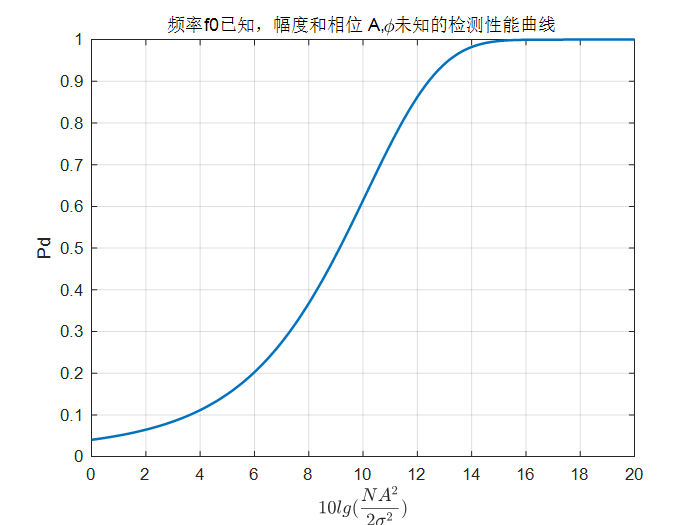
\includegraphics[scale=0.7]{4.1.png}
    \caption{频率\(f_0\)已知,幅度A和相位\(\phi\)未知的检测性能曲线}
    \label{4.1}
\end{figure}

\subsection*{(2)若频率\(f_0\)及幅度相位\(A,\phi \)均未知(假定\(0<f_0<1/2,A>0\)),若\(\sigma^2=1,N=20\),虚警概率设定为\(0.01\),分析检测门限及检测概率并仿真.}

第二问在第一问的基础上更改了初始条件,即频率\(f_0\)未知,推导过程与第一问类似,而\(\alpha_1=\frac{2}{N}\sum_{k=0}^{N-1}z(k)\cos 2\pi f_0k,\alpha_2=\frac{2}{N}\sum_{k=0}^{N-1}z(k)\sin 2\pi f_0k\),这两个量由于\(f_0\)未知,需要遍历\(0<f_0<1/2\)。因此最终用周期图简化判决准则的时候有所不同:
\begin{align*}
    \begin{matrix}
        \max \\f_0
    \end{matrix}
    I(f_0)
    \begin{matrix}
        \mathcal{H}_1 \\
        >             \\
        <             \\
        \mathcal{H}_0
    \end{matrix}
    \sigma^2 \ln \gamma=\gamma^{\prime}
\end{align*}

如果超过判决门限,则判定\(\mathcal{H}_1\),如果周期图峰值超过门限,检测器判存在正选信号,如果是这样,则峰值所处的频率是频率值的最大似然估计。这就解释了为什么周期图或者它的快速傅里叶变换实现几乎是所有窄带检测系统的组成部分。与第一问的差别是虚警率\(P_F\)随搜索频率单元数增加而增加,其中\(L=I(N/2-1)\),I是多普勒单元数,\((N/2-1)\)是距离单元数
\begin{align*}
    P_F=1-(1-\exp(-\frac{\gamma^{\prime}}{\sigma^2}))^L\approx 1-(1-L\exp(-\frac{\gamma^{\prime}}{\sigma^2}))=LP_F(bin)
\end{align*}
假定N点FFT用来计算周期图\(I(f)\),且仅考虑单元扫描,则最大值在频率\(f_k=\frac{k}{N},\quad k=1,2,\ldots, N/2-1\)上求得,我们有
\begin{align*}
    P_D=Q_{\chi^{\prime2}_2(\frac{NA^2}{2\sigma^2})}(2\ln \frac{N/2-1}{P_F})
\end{align*}
检测性能曲线仿真如下:

\begin{figure}[H]
    \centering
    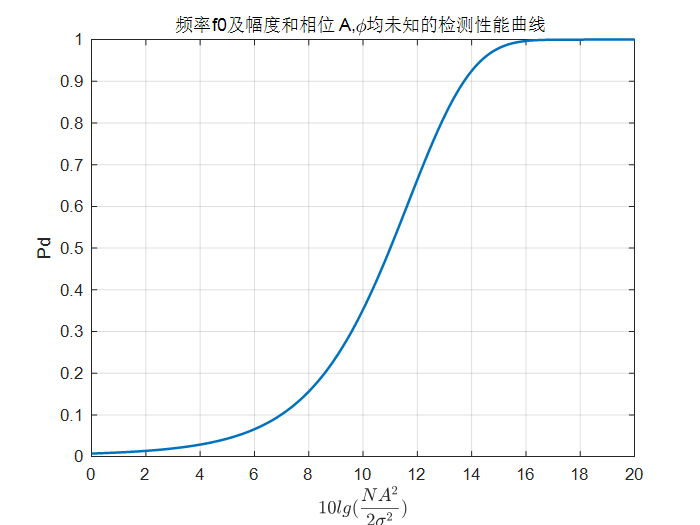
\includegraphics[scale=0.7]{4.2.png}
    \caption{频率\(f_0\),幅度A和相位\(\phi\)均未知的检测性能曲线}
    \label{4.2}
\end{figure}

将第一问与第二问的结果放在一起进行比较:

\begin{figure}[H]
    \centering
    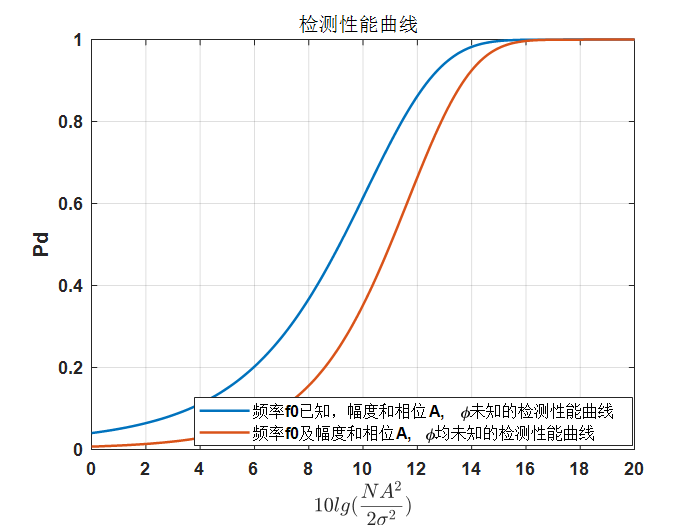
\includegraphics[scale=0.7]{4.3.png}
    \caption{检测性能曲线}
    \label{4.3}
\end{figure}


可见未知参数越多检测性能越差,且对于频率未知的检测而言,N值越大检测性能越大。

\bibliography{books}
\end{document}